\part{C++ advanced}
\chapter{C++ Advanced}
\section{C++ Classes}
\textbf{Formål:} Dette afsnit introducerer objektorienteret programmering (OOP) i C++, herunder klasser, objekter, metoder, Constructors, access specifiers, encapsulation, arv og polymorfisme. Studerende vil lære at bruge OOP-koncepter til at skrive mere struktureret og genanvendelig kode til Arduino-projekter.
\\\\
\noindent\textbf{Læringsmål:} Efter at have læst dette afsnit forventes det, at studerende kan:
\begin{itemize}
	\item Forstå grundlæggende OOP-konceptet og dets anvendelse i Arduino.
	\item Definere og bruge klasser og objekter i Arduino-kode.
	\item Implementere klassemetoder og Constructors i Arduino.
	\item Bruge access specifiers til at kontrollere adgang til klassemedlemmer i Arduino.
	\item Forstå og anvende encapsulation i Arduino-projekter.
	\item Implementere arv og polymorfisme i deres Arduino-programmer.
\end{itemize}

\subsection{C++ Classes/Objects}
\textbf{Teori:} Klasser og objekter er grundlæggende byggesten i objektorienteret programmering (OOP). En klasse er en skabelon eller blueprint for objekter, som definerer de attributter (variabler) og metoder (funktioner), objekterne skal have. En klasse repræsenterer en abstraktion af en ting, hvor tingene har fælles egenskaber og adfærd. Et objekt er en instans af en klasse, hvilket betyder, at det er en konkret manifestation af klassen med specifikke værdier for dets attributter.
\\\\
\noindent OOP gør det muligt at modellere virkelige objekter og deres adfærd på en måde, der gør koden mere struktureret og genanvendelig. Ved at bruge klasser og objekter kan programmører opdele komplekse problemer i mindre, håndterbare enheder, hvilket letter både udvikling og vedligeholdelse af koden.
\\\\
\noindent\noindent\textbf{Eksempel:}
\begin{lstlisting}[language=C++]
	class LED {
		int pin;
		
		public:
		LED(int p) {
			pin = p;
			pinMode(pin, OUTPUT);
		}
		
		void on() {
			digitalWrite(pin, HIGH);
		}
		
		void off() {
			digitalWrite(pin, LOW);
		}
	};
	
	LED led1(13); // create an object of class LED
	
	void setup() {
	}
	
	void loop() {
		led1.on();
		delay(1000);
		led1.off();
		delay(1000);
	}
\end{lstlisting}
\begin{figure}[h!]
	\centering
	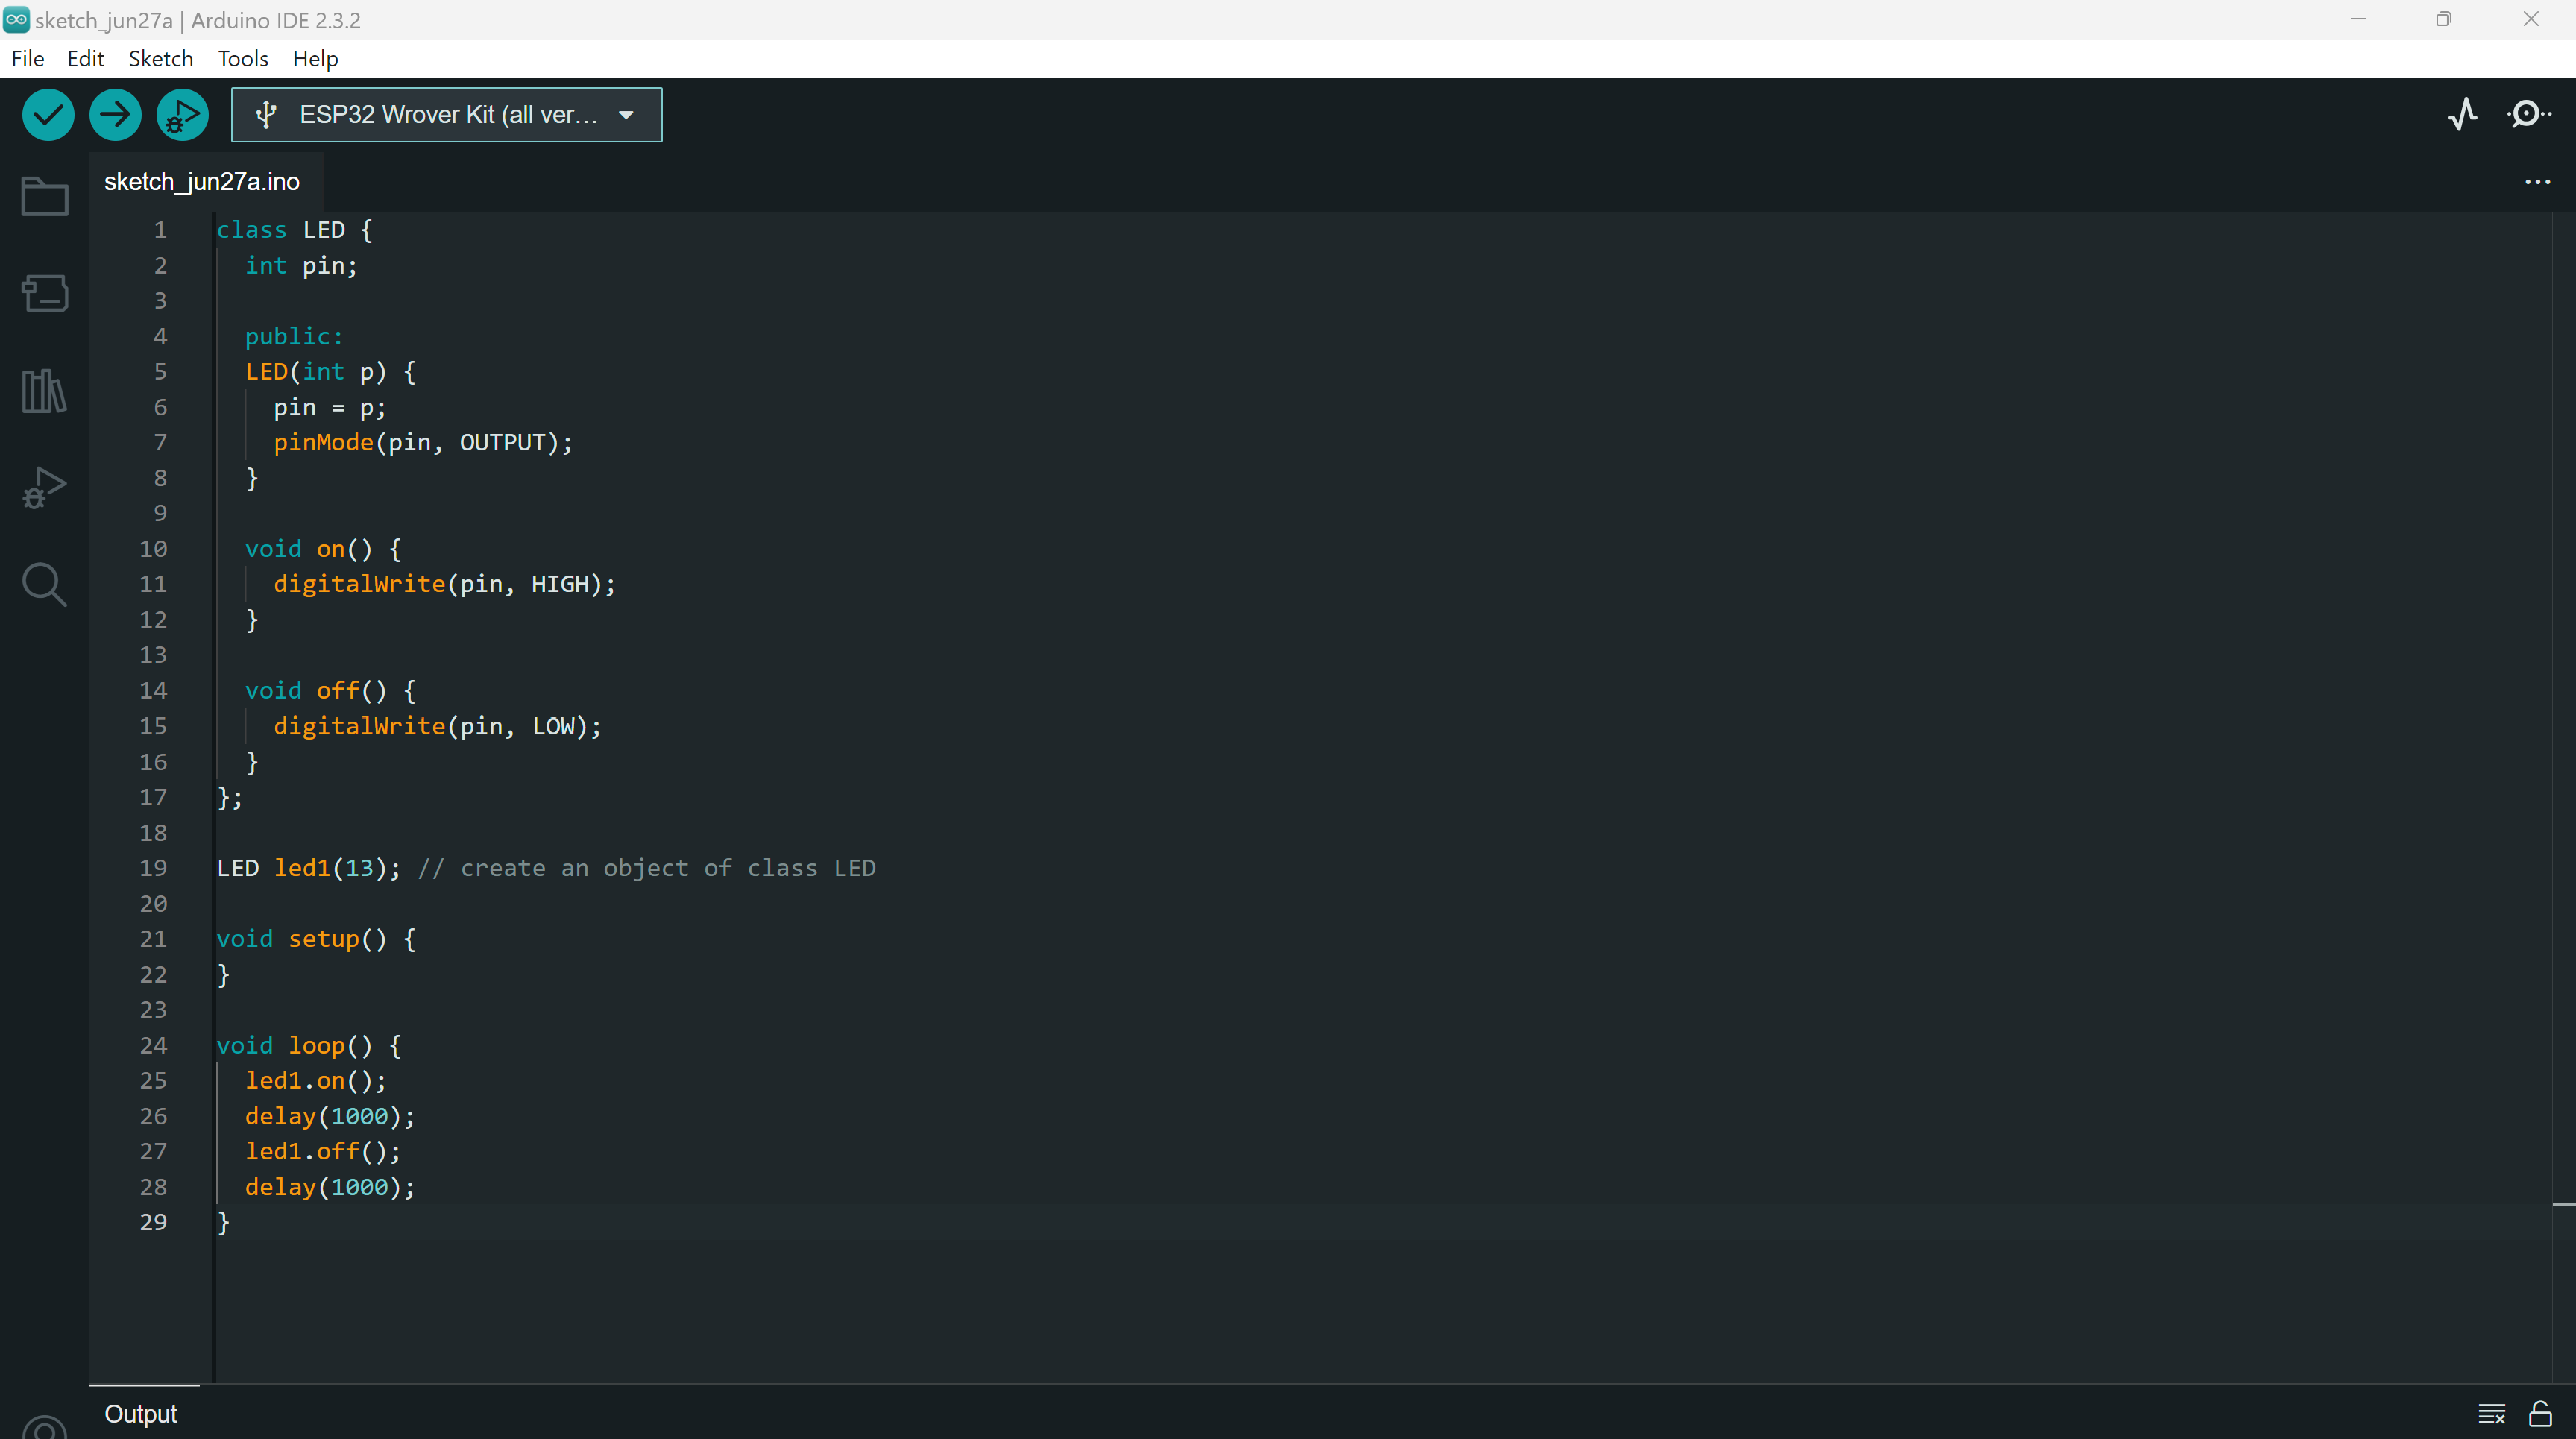
\includegraphics[width=\textwidth]{fig/fig13.png}
	\caption{text}
	\label{fig:13}
\end{figure}

\subsection{C++ Class Methods}
\textbf{Teori:} Metoder er funktioner, der er defineret inde i en klasse. De bruges til at definere adfærd for objekter. Metoder kan manipulere objektets tilstand og udføre opgaver baseret på objektets data. Metoder kan have adgang til objektets data via \texttt{this} pegeren, som implicit henviser til det kaldende objekt.
\\\\
\noindent Metoder kan være offentlige (\texttt{public}) eller private (\texttt{private}), hvilket kontrollerer deres synlighed og adgang fra udenfor klassen. Offentlige metoder er en del af klassens offentlige grænseflade, mens private metoder kun kan kaldes fra indenfor klassen selv.
\\\\
\noindent\textbf{Eksempel:}
\begin{lstlisting}[language=C++]
	class LED {
		int pin;
		
		public:
		LED(int p) {
			pin = p;
			pinMode(pin, OUTPUT);
		}
		
		void on() {
			digitalWrite(pin, HIGH);
		}
		
		void off() {
			digitalWrite(pin, LOW);
		}
	};
	
	LED led1(13);
	
	void setup() {
	}
	
	void loop() {
		led1.on();
		delay(1000);
		led1.off();
		delay(1000);
	}
\end{lstlisting}
\begin{figure}[h!]
	\centering
	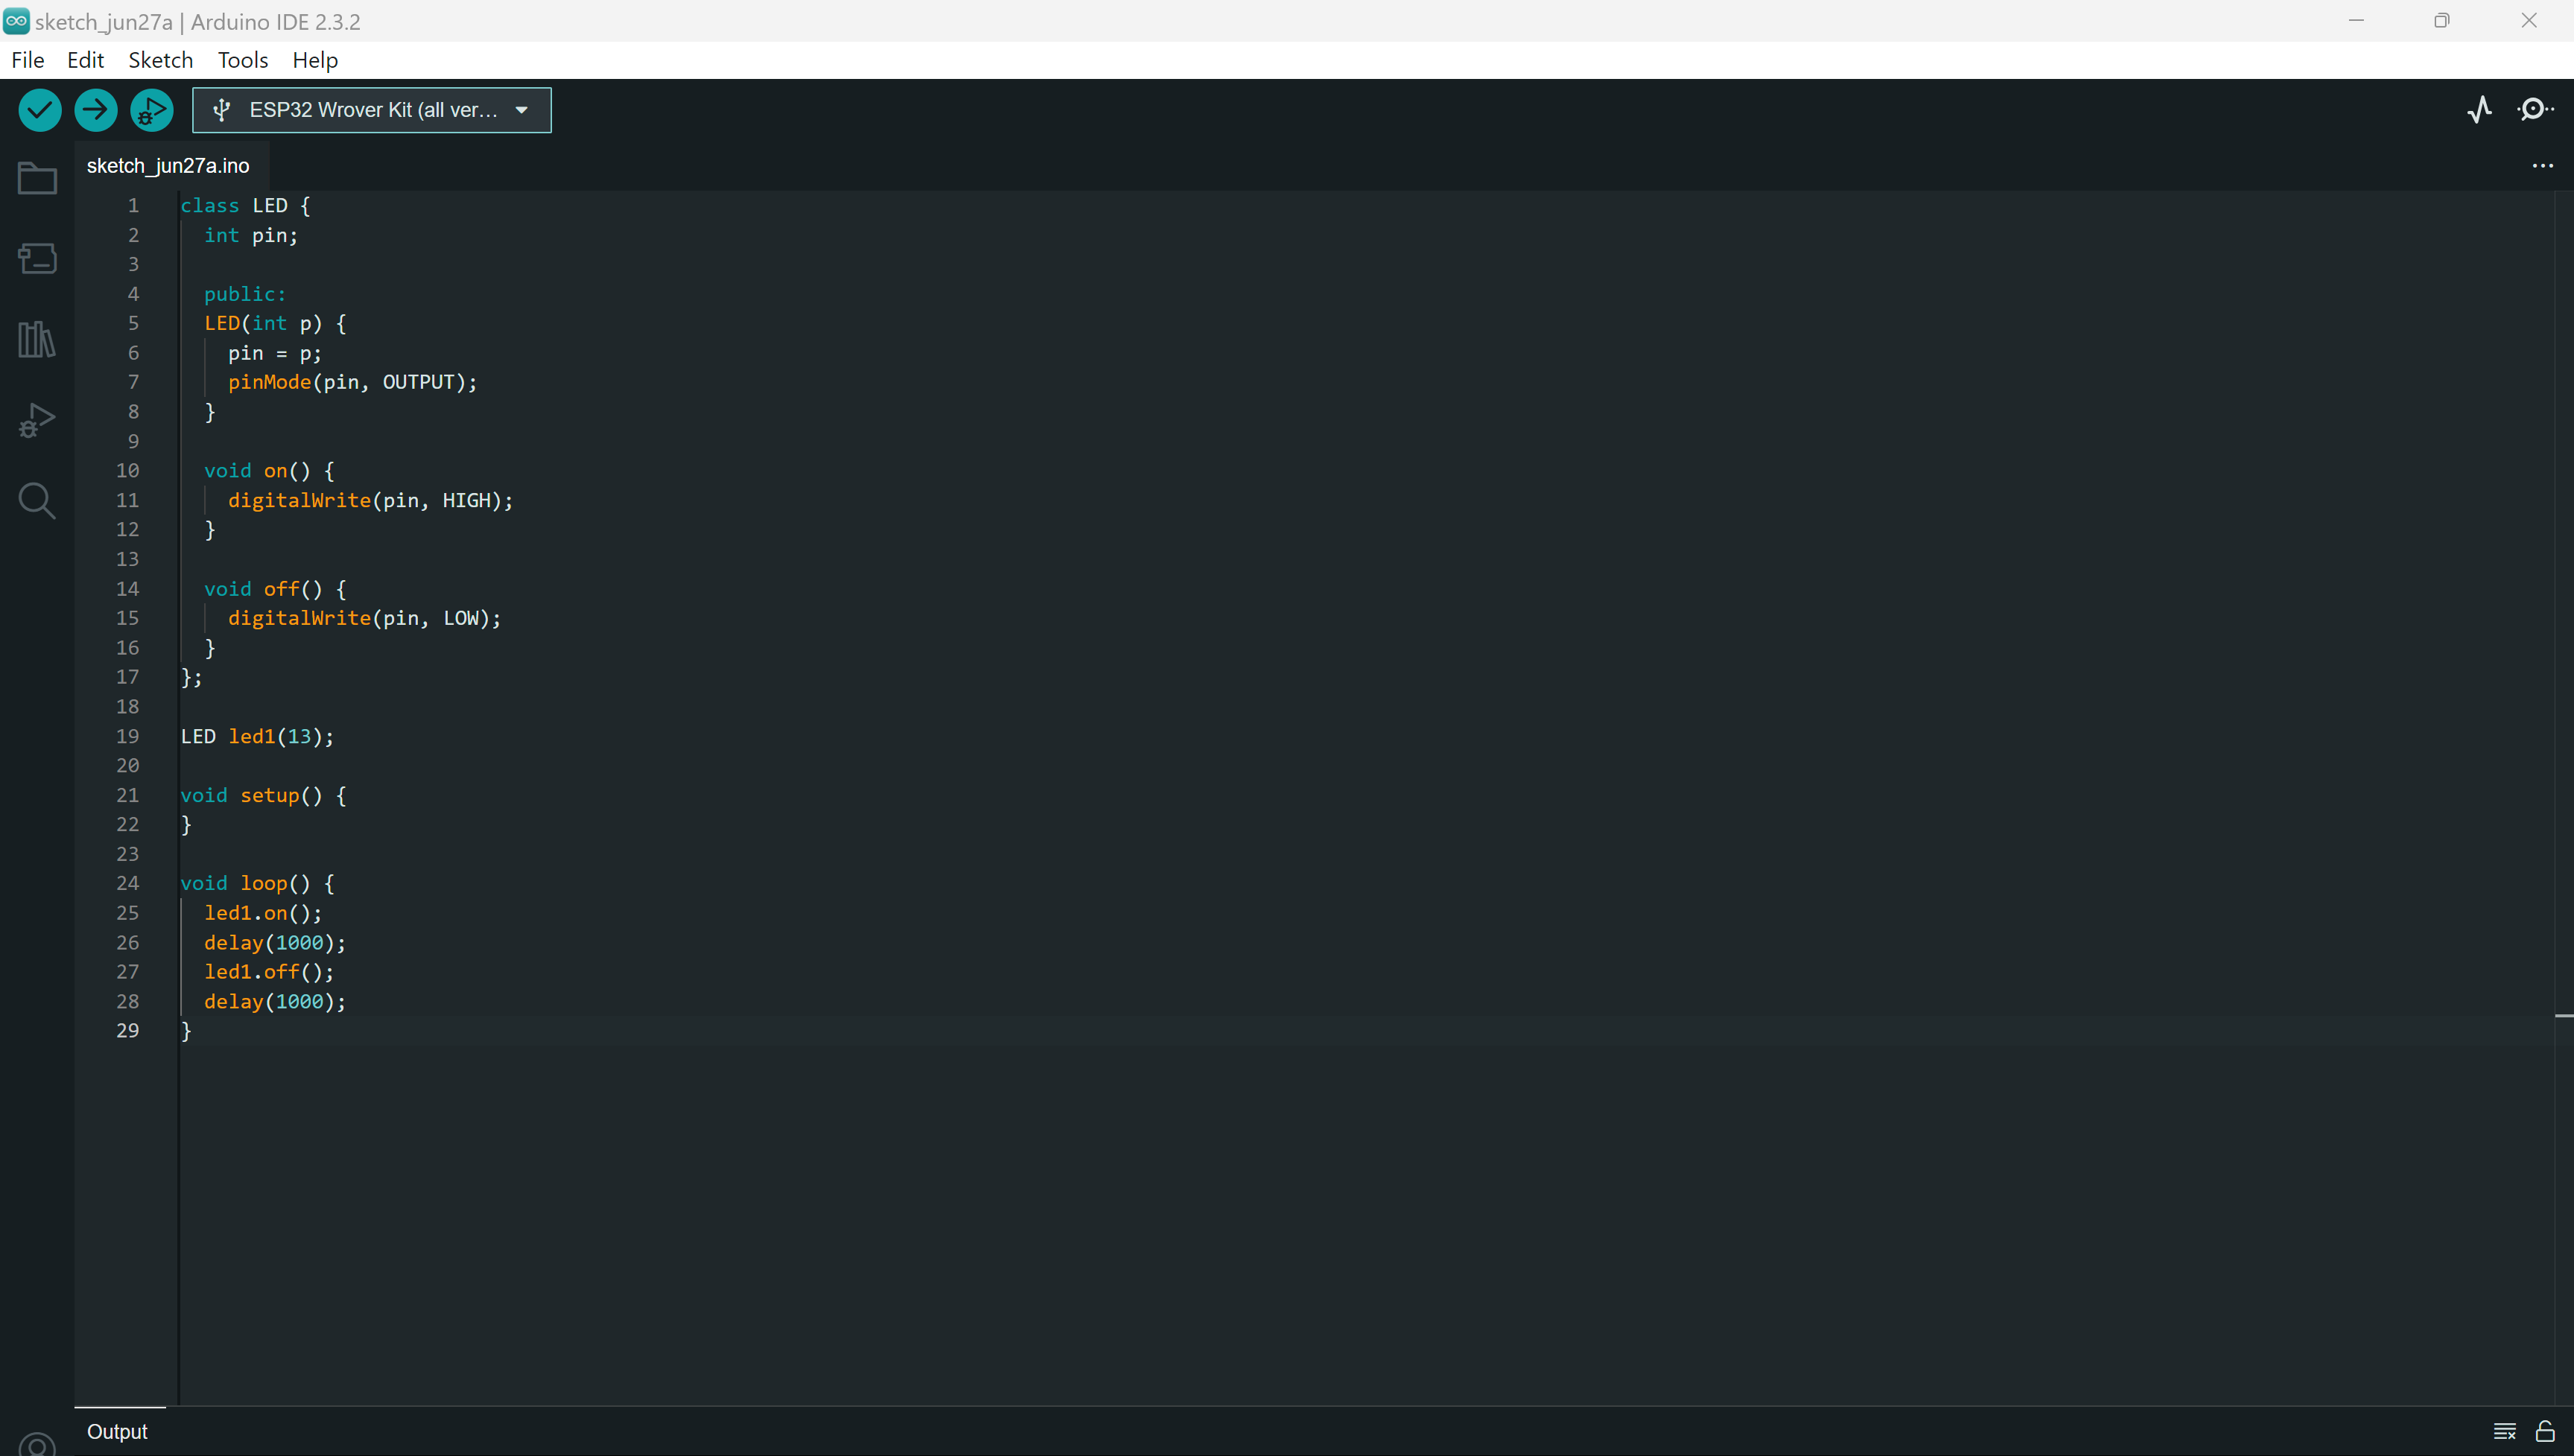
\includegraphics[width=\textwidth]{fig/fig18.png}
	\caption{C++ Class Methods}
	\label{fig:18}
\end{figure}


\subsection{C++ Constructors}
\textbf{Teori:} Constructors er specielle metoder, der kaldes automatisk, når et objekt skabes. De bruges til at initialisere objektets egenskaber. Constructors har samme navn som klassen og har ingen returtype. Constructors kan også tage parametre, som kan bruges til at initialisere objektets data med specifikke værdier ved skabelsen.
\\\\
\noindent En korrekt brug af Constructors er vigtig for at sikre, at objekter altid starter i en gyldig tilstand. Desuden kan Constructors også bruges til at allokere ressourcer, som objektet har brug for i sin levetid.
\\\\
\noindent\textbf{Eksempel:}
\begin{lstlisting}[language=C++]
	class LED {
		int pin;
		
		public:
		LED(int p) {
			pin = p;
			pinMode(pin, OUTPUT);
		}
		
		void on() {
			digitalWrite(pin, HIGH);
		}
		
		void off() {
			digitalWrite(pin, LOW);
		}
	};
	
	LED led1(13); // constructor is called here
	
	void setup() {
	}
	
	void loop() {
		led1.on();
		delay(1000);
		led1.off();
		delay(1000);
	}
\end{lstlisting}
\begin{figure}[h!]
	\centering
	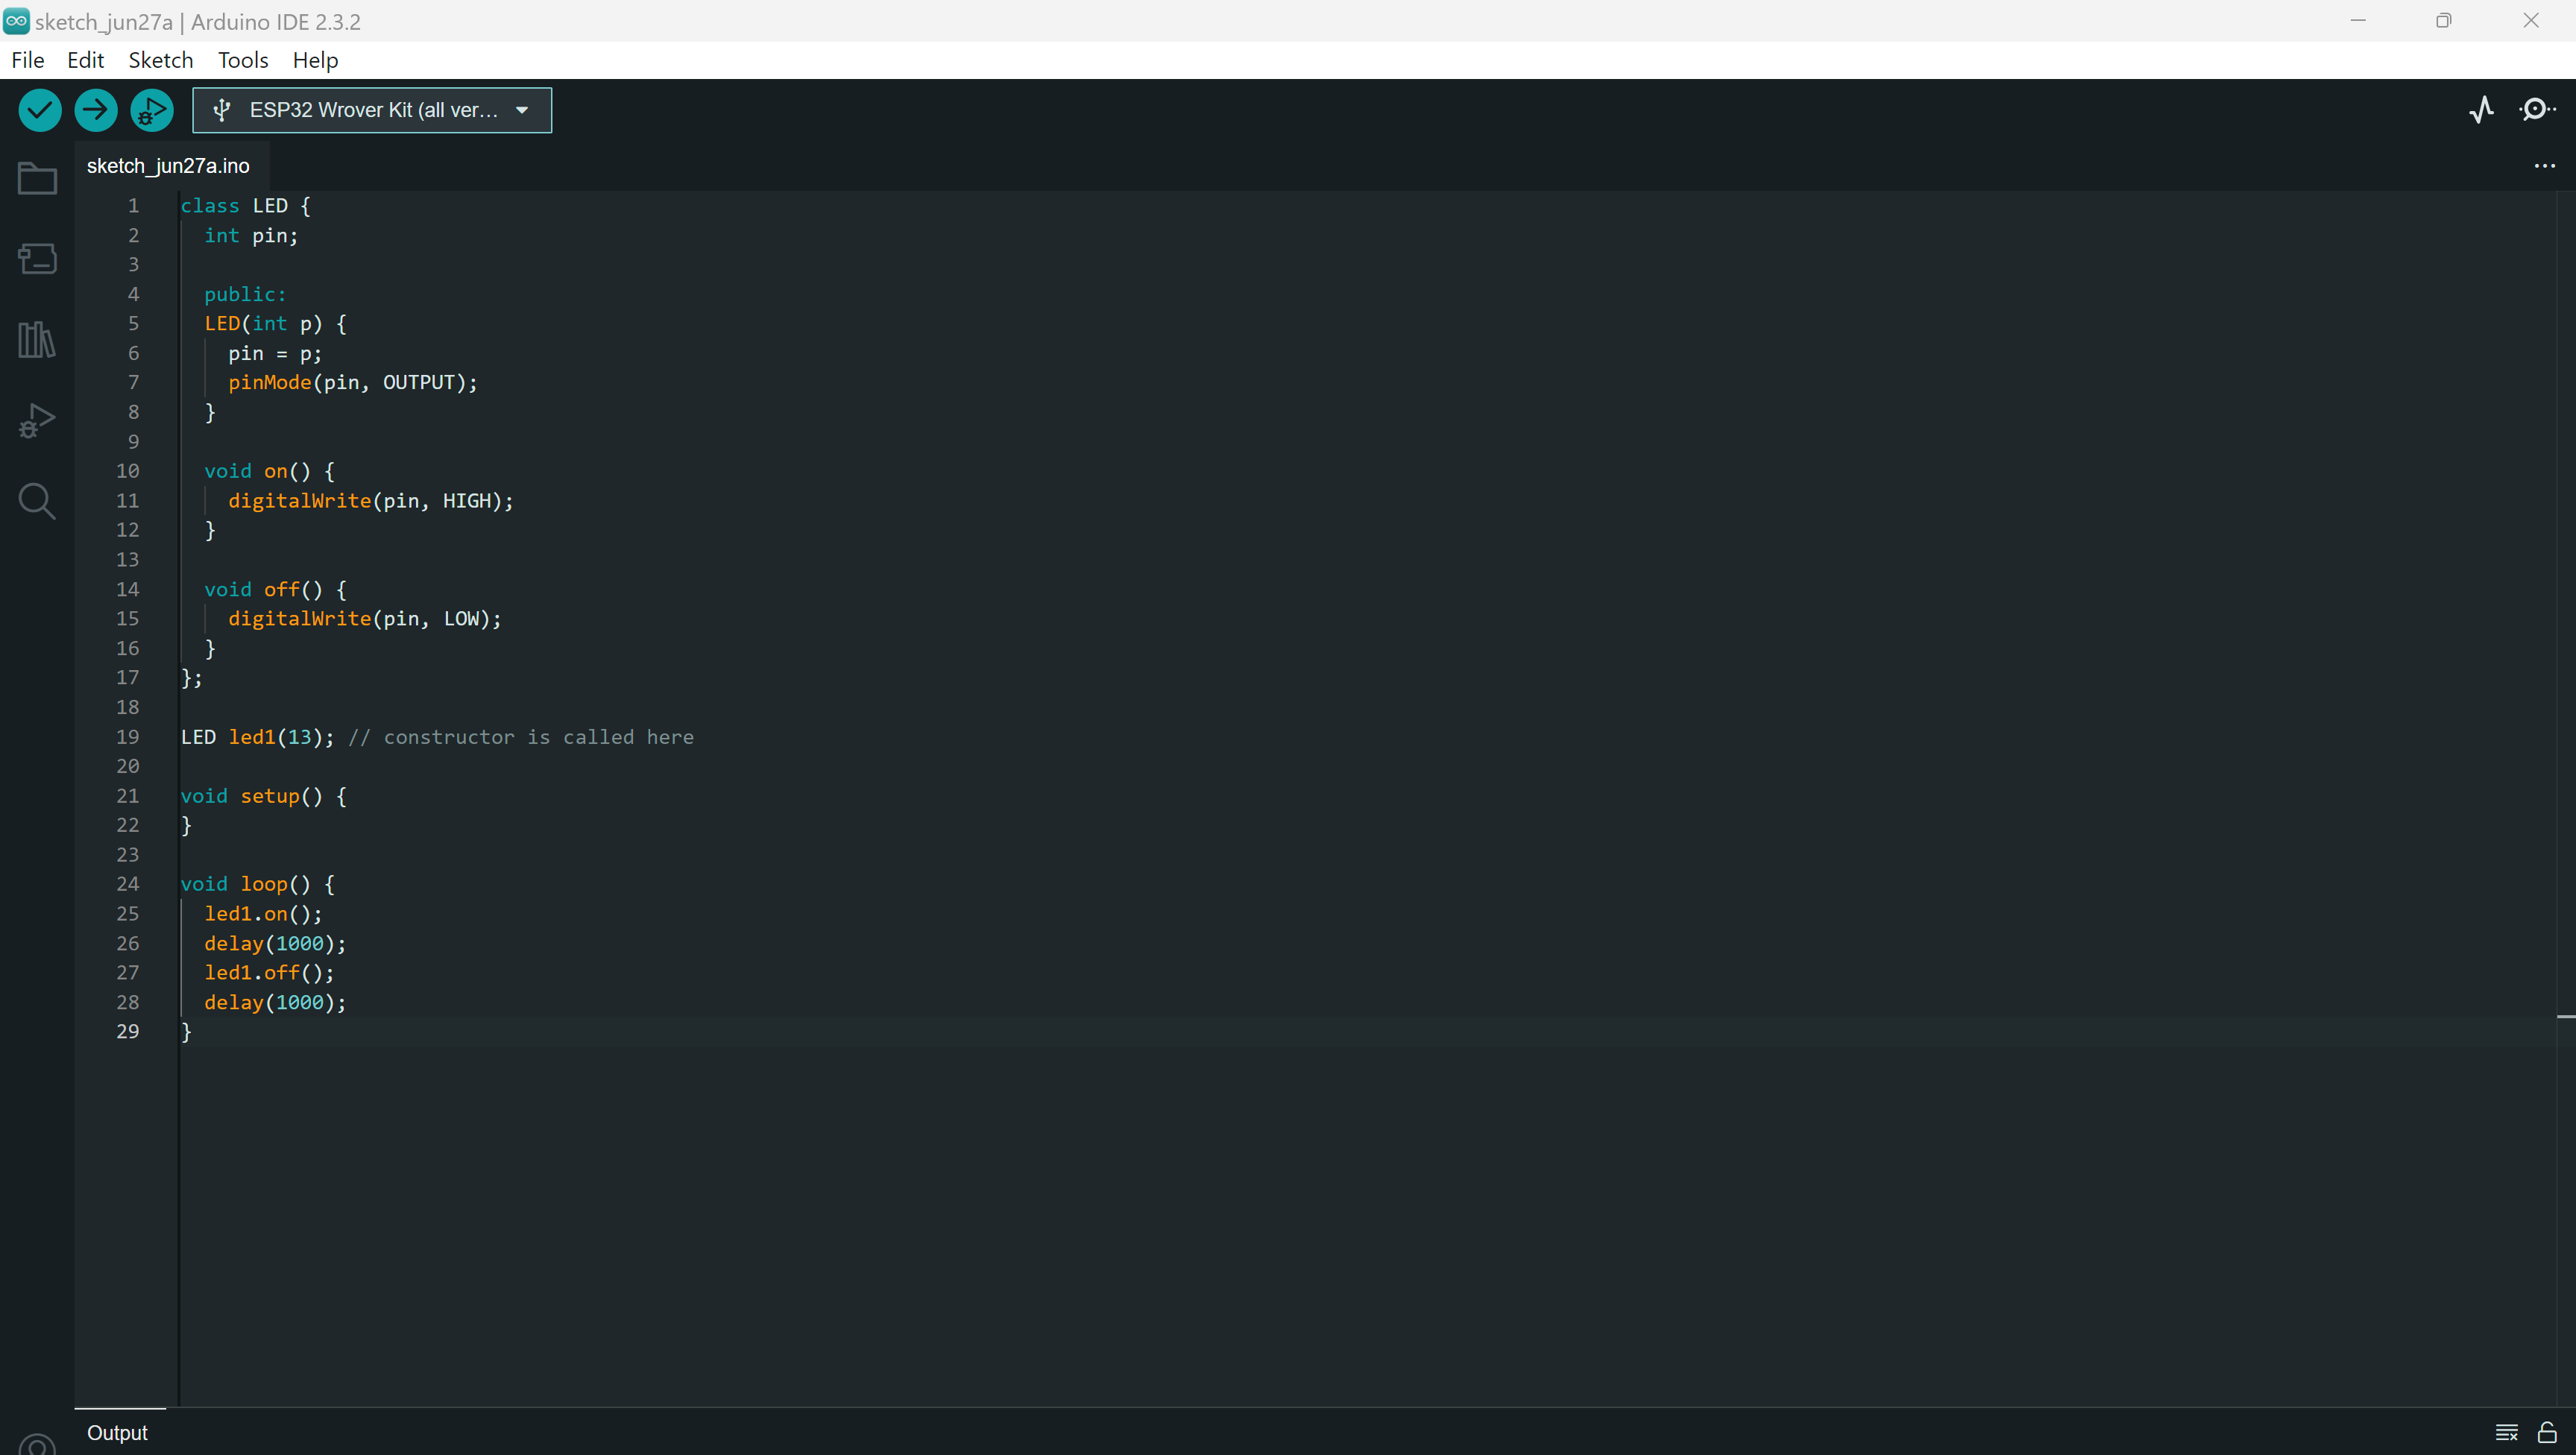
\includegraphics[width=\textwidth]{fig/fig17.png}
	\caption{C++ Constructors}
	\label{fig:17}
\end{figure}

\subsection{C++ Access Specifiers}
\textbf{Teori:} Access specifiers kontrollerer adgangen til klassemedlemmer. De mest almindelige access specifiers er \texttt{public}, \texttt{private}, og \texttt{protected}. \texttt{public} medlemmer kan tilgås fra enhver kode, mens \texttt{private} medlemmer kun kan tilgås fra indenfor klassen selv. \texttt{protected} medlemmer kan tilgås fra klassen og dens subklasser, men ikke fra andre dele af programmet.
\\\\
\noindent Access specifiers er en vigtig del af encapsulation, en OOP-praksis, der hjælper med at beskytte data og funktioner inde i en klasse fra utilsigtet eller skadelig adgang og ændring.
\\\\
\noindent\noindent\textbf{Eksempel:}
\begin{lstlisting}[language=C++]
	class LED {
		private:
		int pin;
		
		public:
		LED(int p) {
			pin = p;
			pinMode(pin, OUTPUT);
		}
		
		void on() {
			digitalWrite(pin, HIGH);
		}
		
		void off() {
			digitalWrite(pin, LOW);
		}
	};
	
	LED led1(13);
	
	void setup() {
	}
	
	void loop() {
		led1.on();
		delay(1000);
		led1.off();
		delay(1000);
	}
\end{lstlisting}
\begin{figure}[h!]
	\centering
	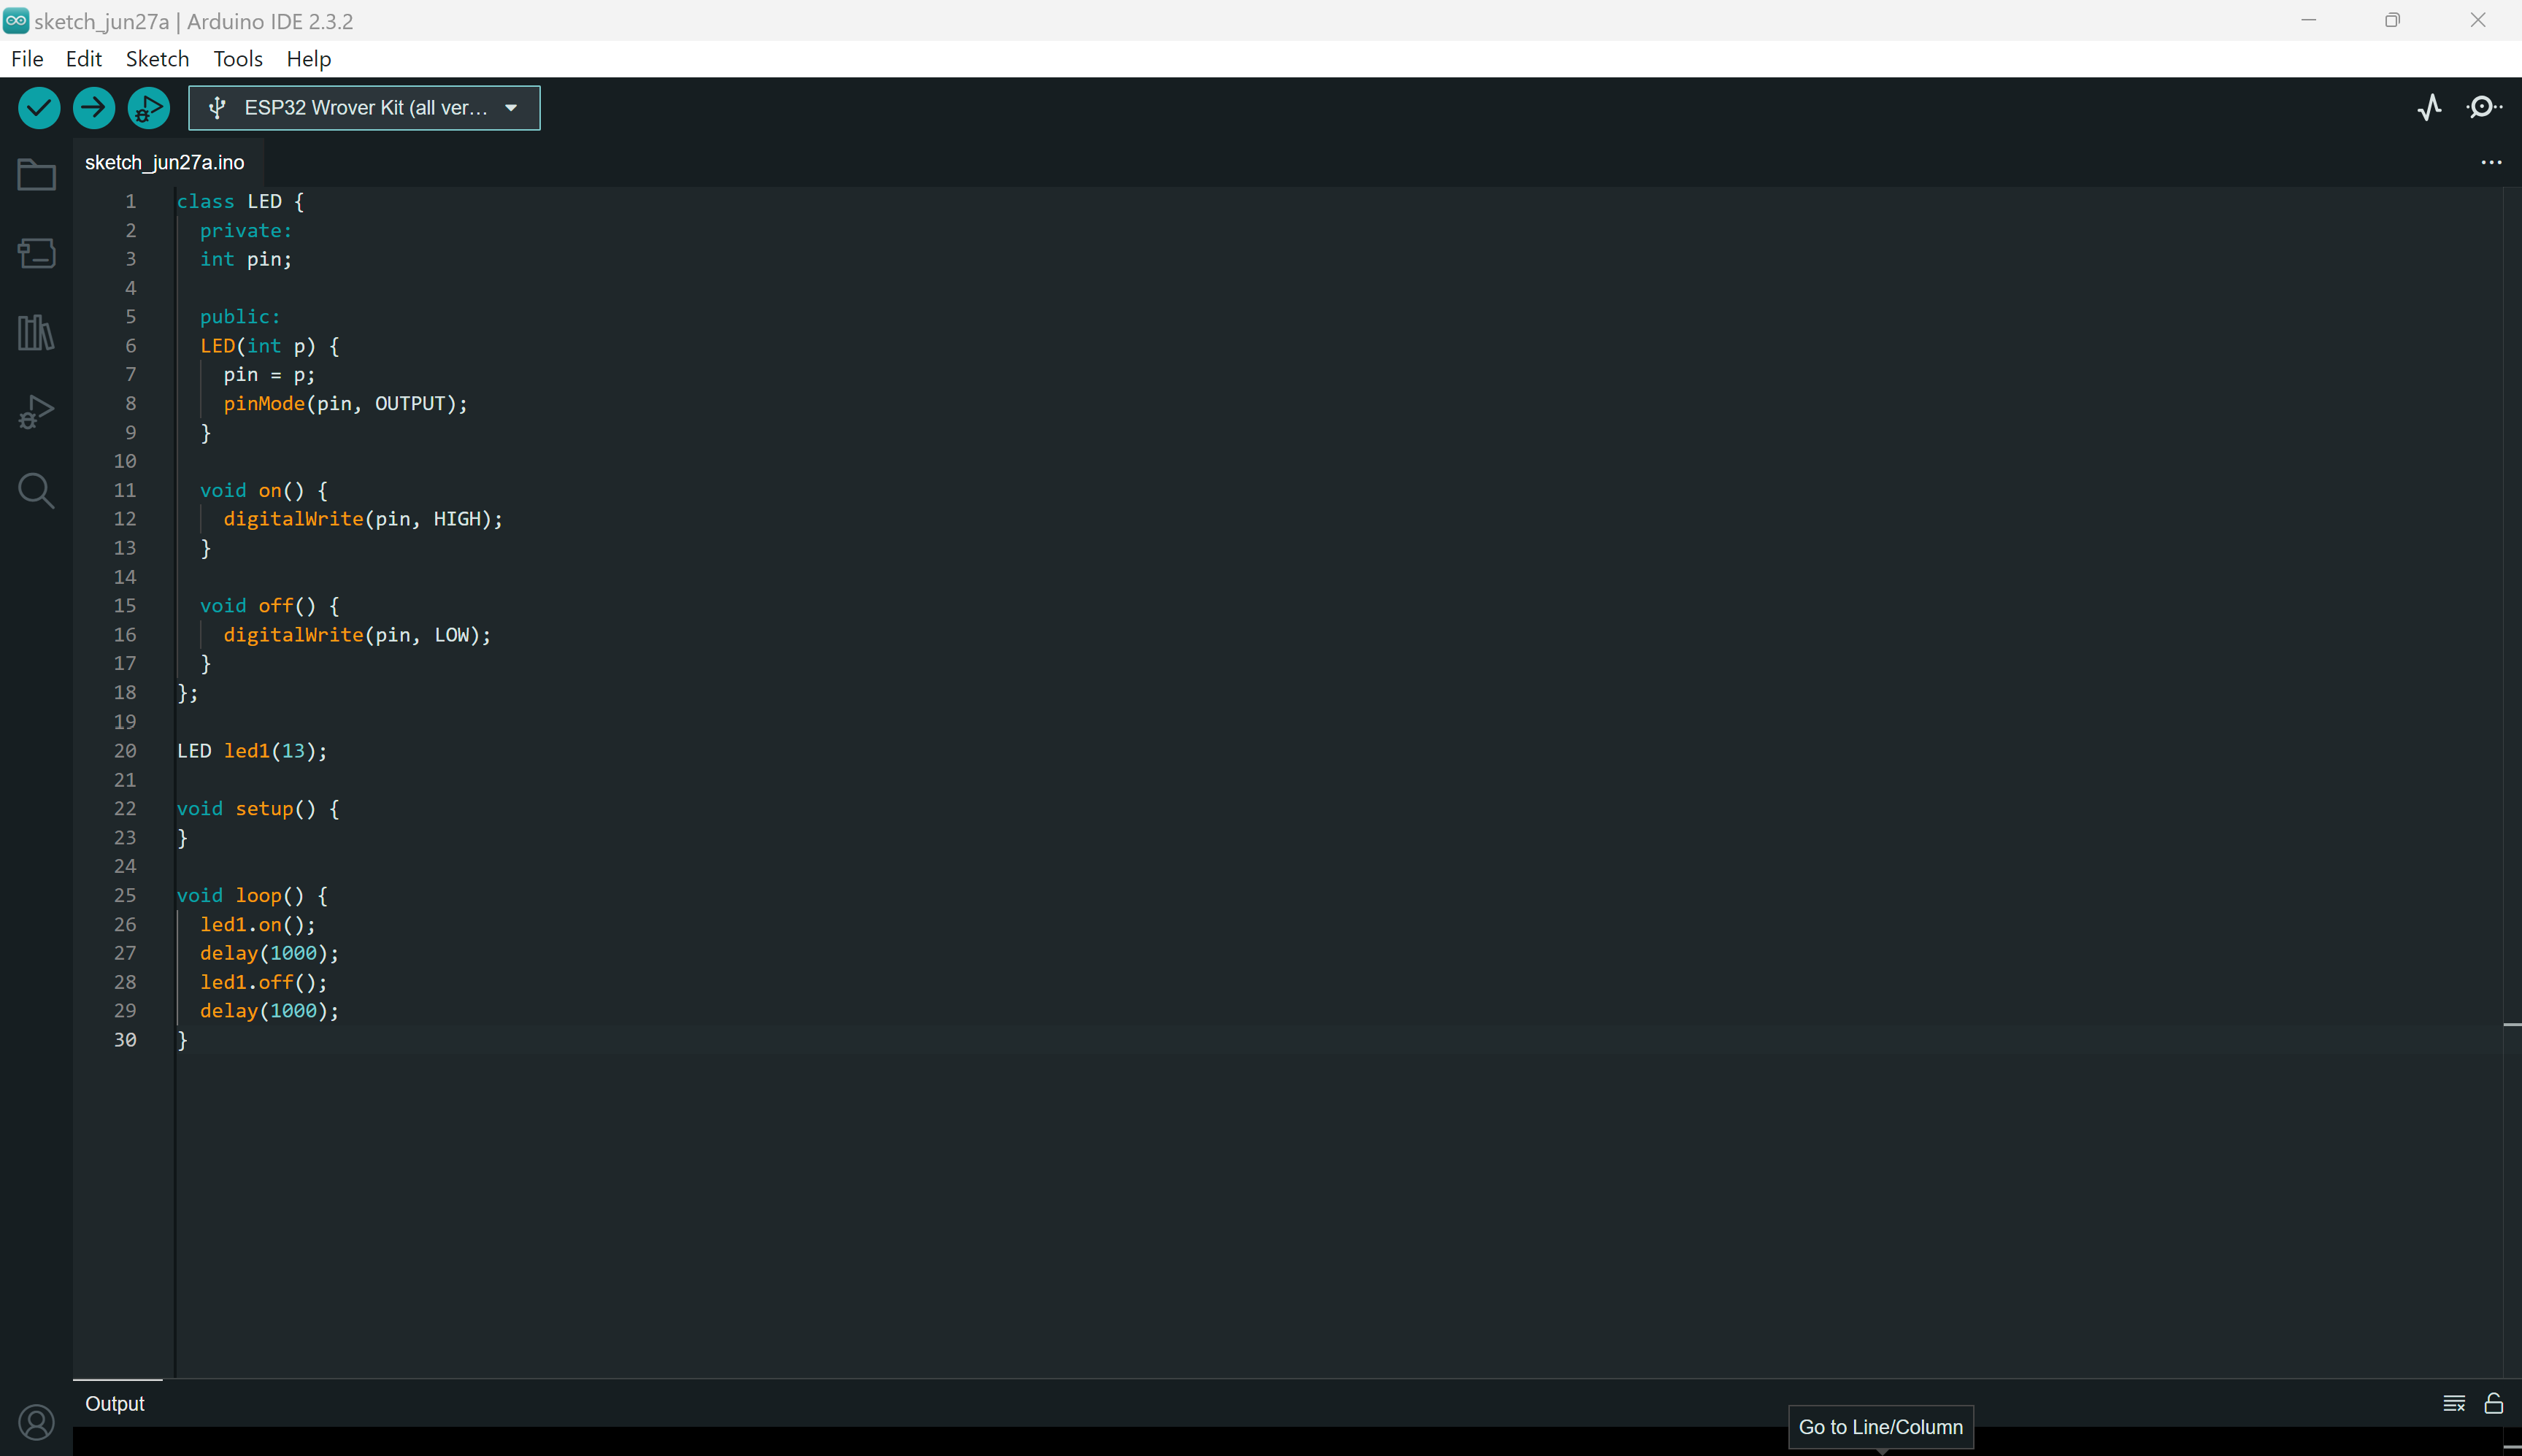
\includegraphics[width=\textwidth]{fig/fig16.png}
	\caption{C++ Access Specifiers}
	\label{fig:16}
\end{figure}

\subsection{C++ Encapsulation}
\textbf{Teori:} Encapsulation er processen med at skjule data implementeringsdetaljer og beskytte mod uautoriseret adgang. Det opnås ved hjælp af private medlemmer og offentlige metoder. Encapsulation sikrer data integritet og gør koden mere robust og vedligeholdelsesvenlig. Ved at skjule objektets indre detaljer kan udviklere ændre implementeringen uden at påvirke andre dele af programmet, som afhænger af objektets grænseflade.
\\\\
\noindent Encapsulation gør det muligt at skabe en klar og veldefineret grænseflade for en klasse, hvilket gør det lettere at bruge og forstå klassen uden at kende dens indre detaljer. Det fremmer også genbrug af kode og modularitet.
\\\\
\noindent\noindent\textbf{Eksempel:}
\begin{lstlisting}[language=C++]
	class LED {
		private:
		int pin;
		
		public:
		LED(int p) {
			pin = p;
			pinMode(pin, OUTPUT);
		}
		
		void on() {
			digitalWrite(pin, HIGH);
		}
		
		void off() {
			digitalWrite(pin, LOW);
		}
	};
	
	LED led1(13);
	
	void setup() {
	}
	
	void loop() {
		led1.on();
		delay(1000);
		led1.off();
		delay(1000);
	}
\end{lstlisting}
\begin{figure}[h!]
	\centering
	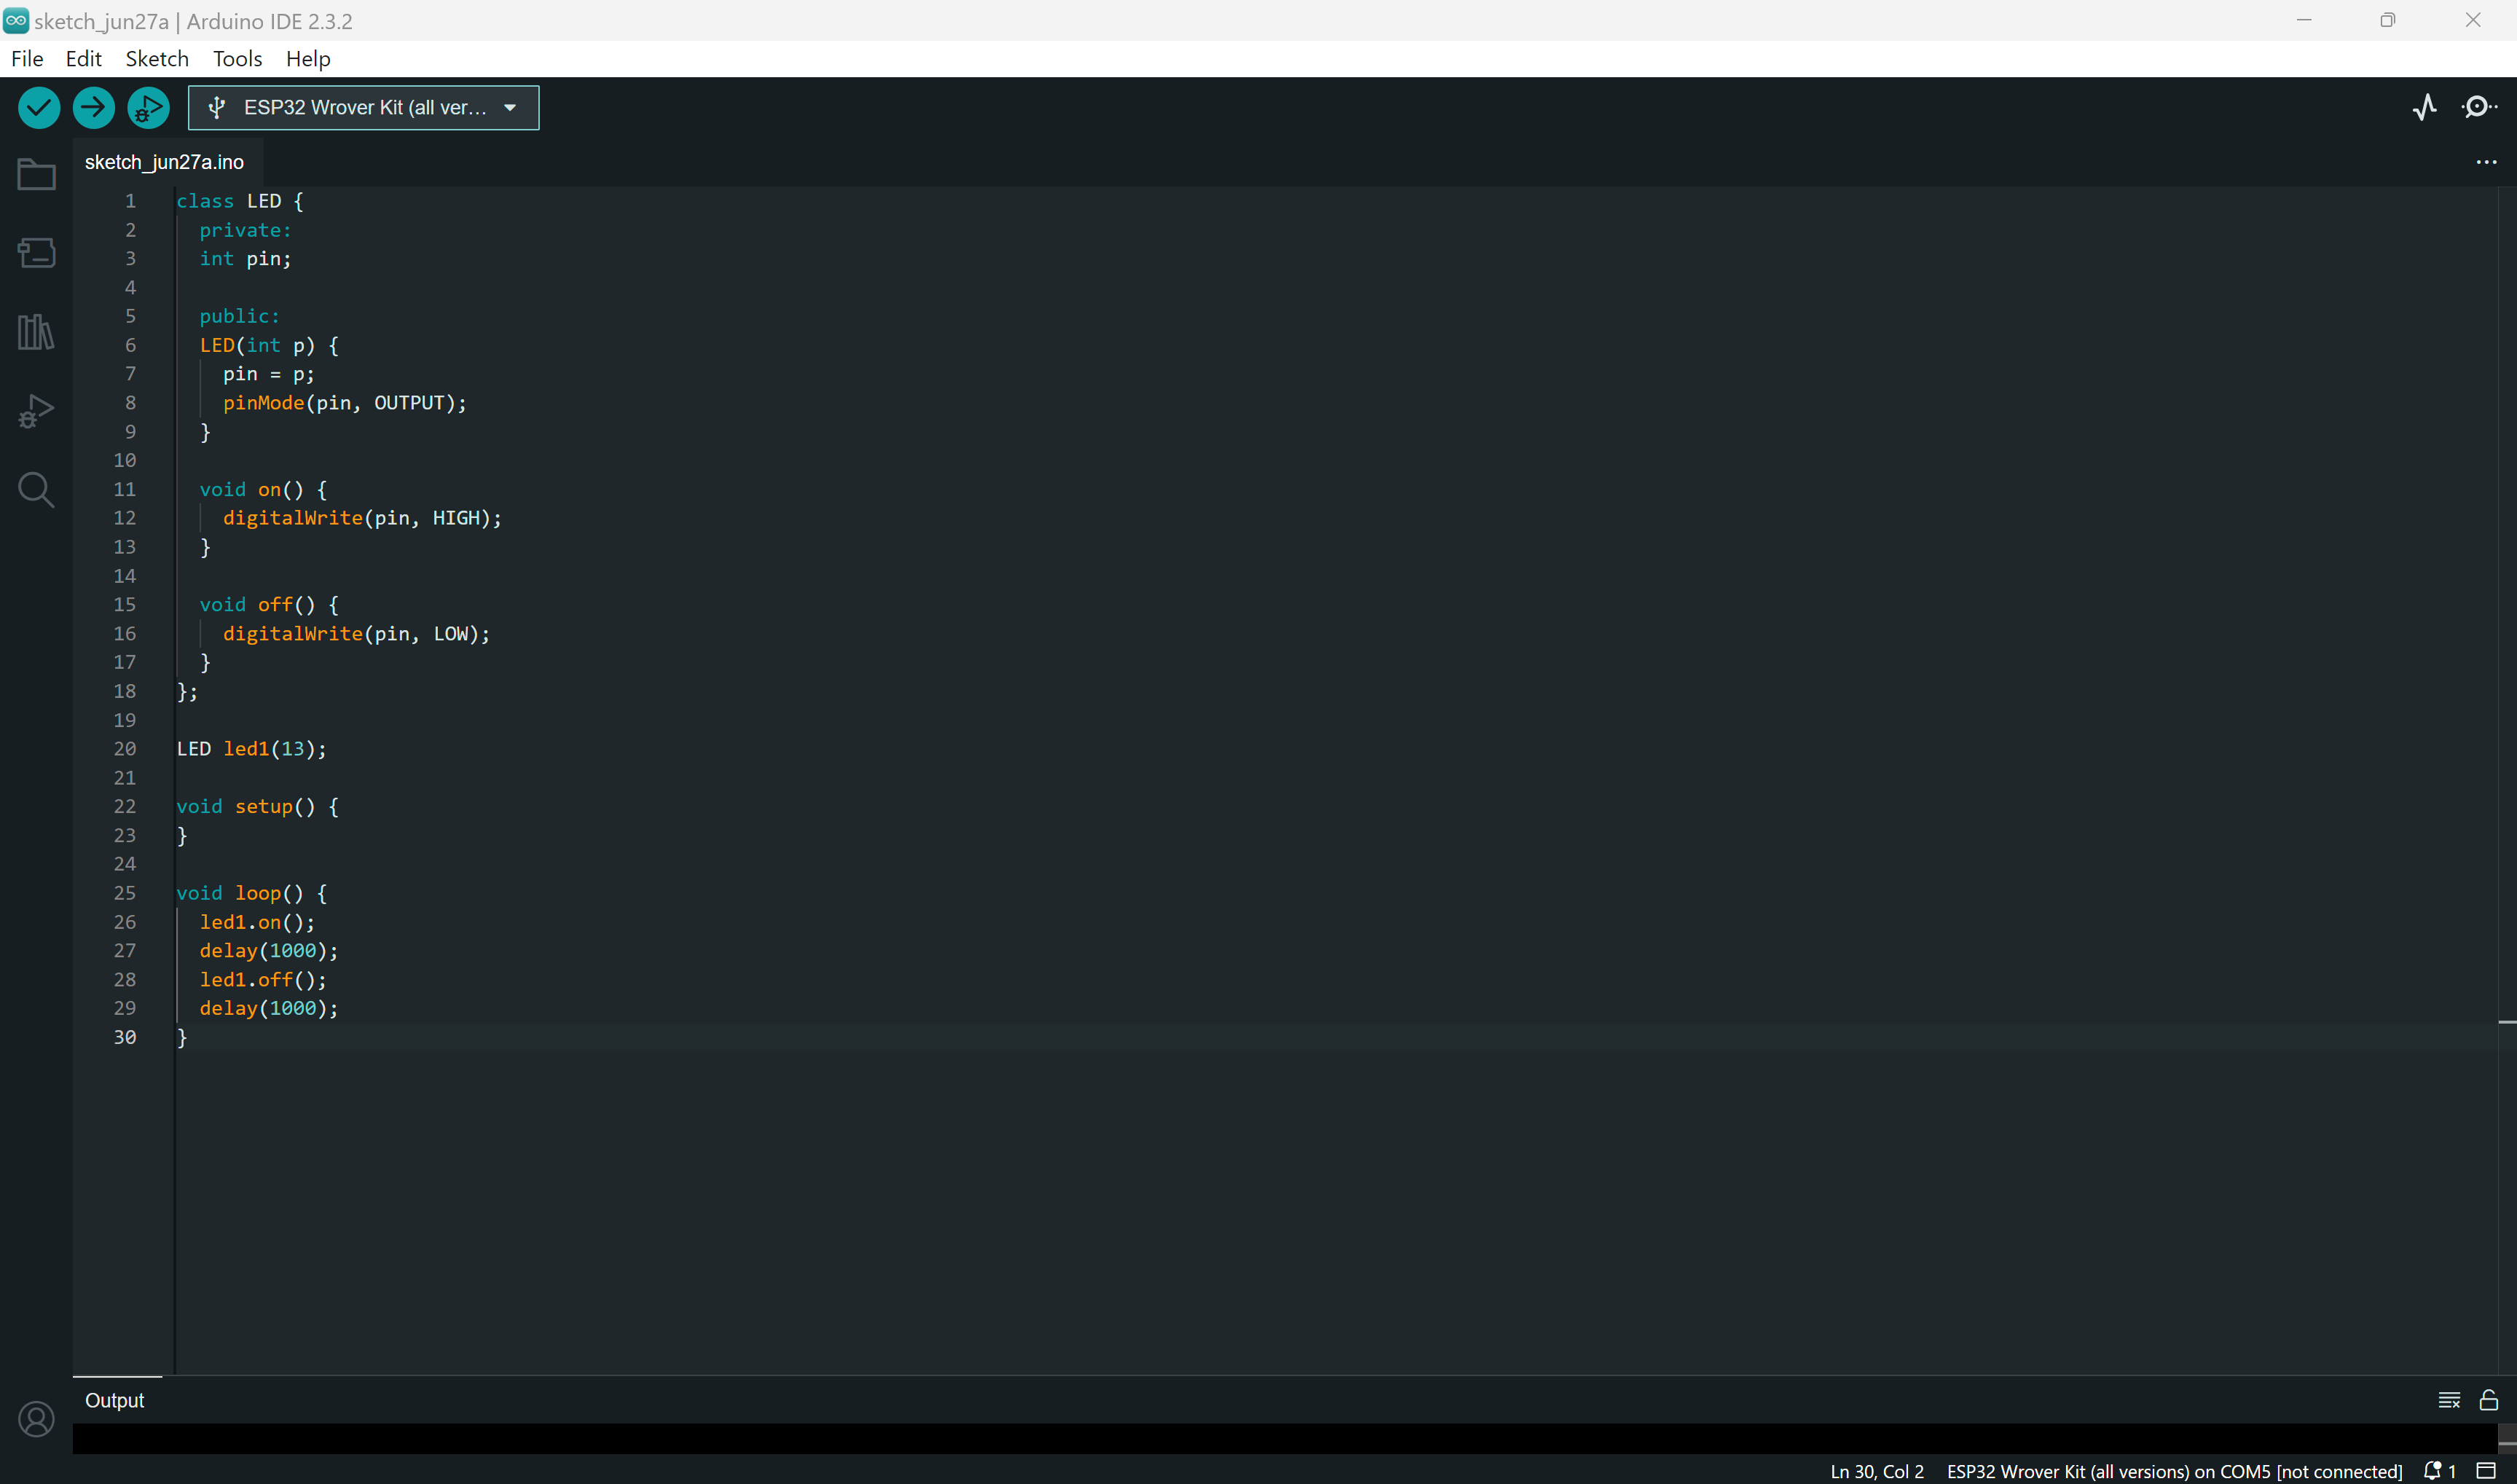
\includegraphics[width=\textwidth]{fig/fig15.png}
	\caption{C++ Encapsulation}
	\label{fig:15}
\end{figure}

\subsection{C++ Inheritance}
\textbf{Teori:} Arv tillader en klasse at arve egenskaber og metoder fra en anden klasse. Dette fremmer genbrug og struktureret kode. En baseklasse (eller superklasse) kan have flere afledte klasser (eller subklasser), som nedarver baseklassens medlemmer og metoder. Afledte klasser kan også tilføje deres egne medlemmer og metoder eller overskrive baseklassens metoder.
\\\\
\noindent Arv bruges til at skabe en hierarkisk struktur og dele funktionalitet på tværs af klasser. Det tillader udviklere at bygge komplekse systemer ved at genbruge og udvide eksisterende kode. Arv understøtter også polymorfisme, hvor objekter af forskellige klasser kan behandles ens, hvis de deler samme baseklasse.
\\\\
\noindent\textbf{Eksempel:}
\begin{lstlisting}[language=C++]
	class LED {
		protected:
		int pin;
		
		public:
		LED(int p) {
			pin = p;
			pinMode(pin, OUTPUT);
		}
		
		void on() {
			digitalWrite(pin, HIGH);
		}
		
		void off() {
			digitalWrite(pin, LOW);
		}
	};
	
	class BlinkingLED : public LED {
		public:
		BlinkingLED(int p) : LED(p) {}
		
		void blink() {
			on();
			delay(500);
			off();
			delay(500);
		}
	};
	
	BlinkingLED led1(13);
	
	void setup() {
	}
	
	void loop() {
		led1.blink();
	}
\end{lstlisting}
\begin{figure}[h!]
	\centering
	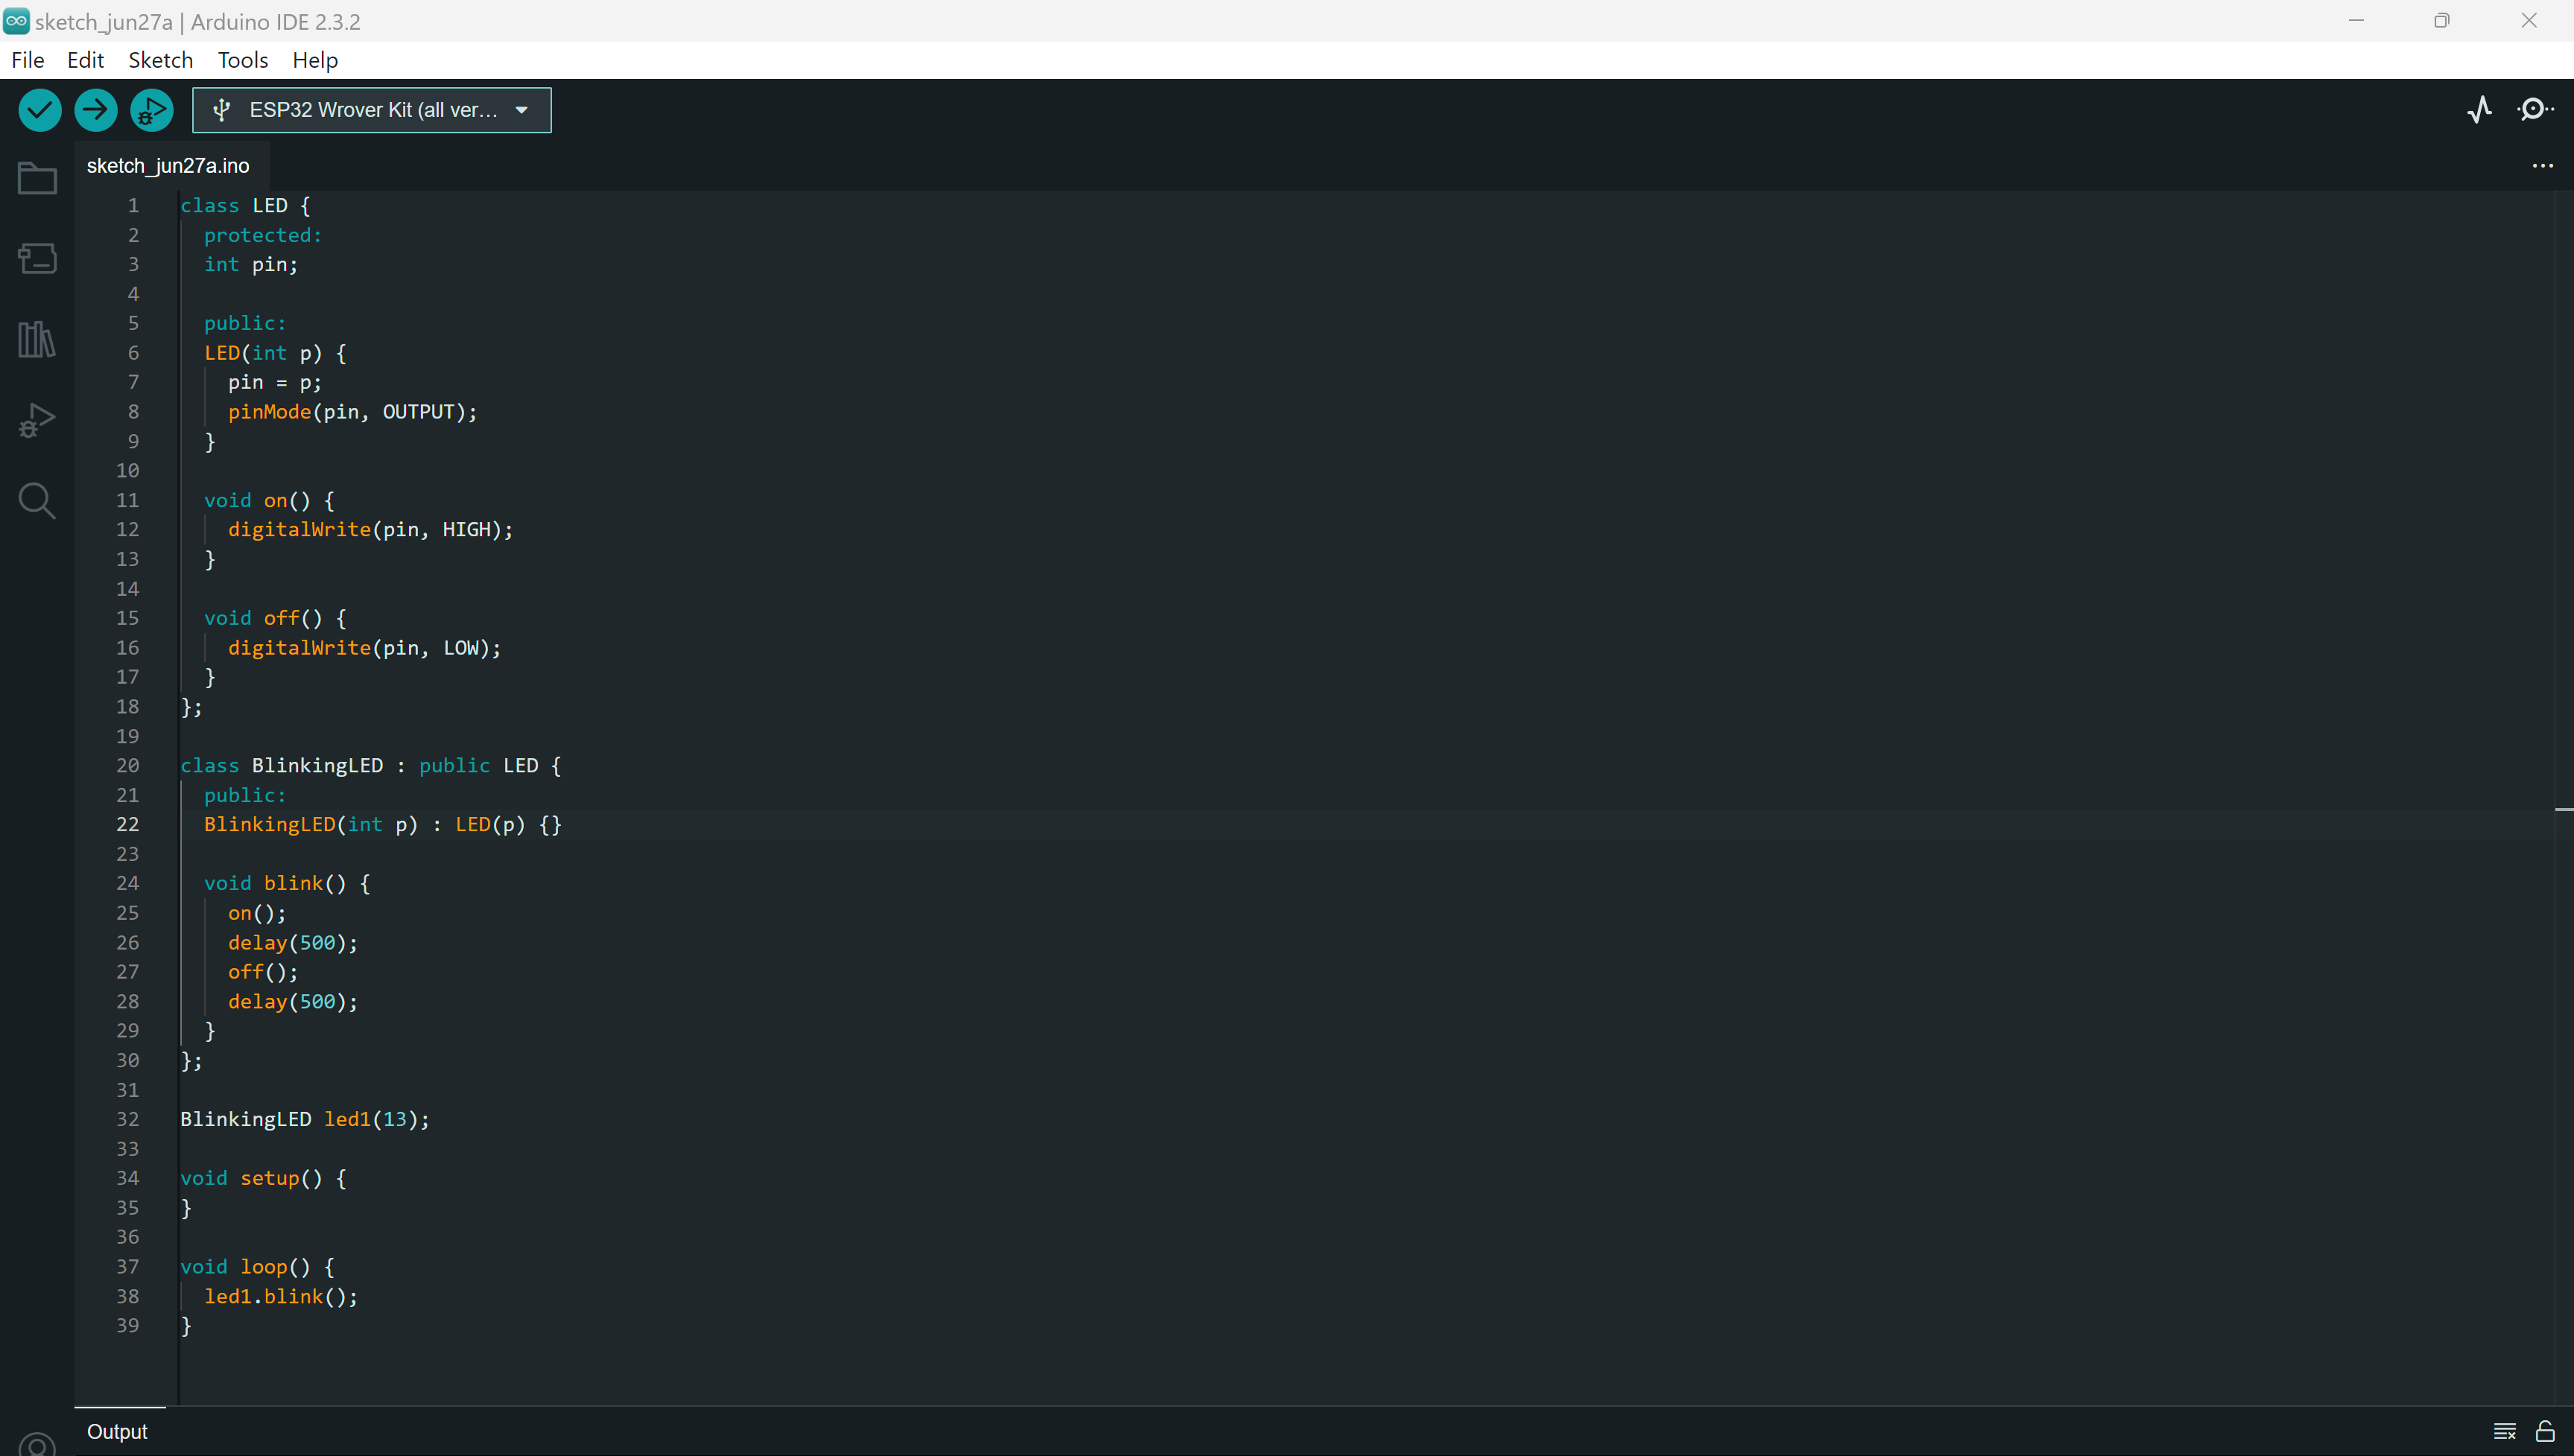
\includegraphics[width=\textwidth]{fig/fig14.png}
	\caption{C++ Inheritance}
	\label{fig:14}
\end{figure}

\subsection{C++ Polymorphism}
\textbf{Teori:} Polymorfisme tillader metoder at have forskellige implementeringer, selv når de deler samme navn. Dette opnås gennem virtual funktioner og arv. Virtual funktioner tillader afledte klasser at overskrive baseklassens funktioner, hvilket gør det muligt at kalde forskellige implementeringer afhængigt af objektets type.
\\\\
\noindent Polymorfisme gør det muligt at skrive fleksibel og udvidelig kode. Det tillader en funktion at håndtere objekter af forskellige typer på en ensartet måde, hvilket reducerer kompleksiteten og øger genanvendeligheden af koden.
\\\\
\noindent\textbf{Eksempel:}
\begin{lstlisting}[language=C++]
	class LED {
		protected:
		int pin;
		
		public:
		LED(int p) {
			pin = p;
			pinMode(pin, OUTPUT);
		}
		
		virtual void on() {
			digitalWrite(pin, HIGH);
		}
		
		virtual void off() {
			digitalWrite(pin, LOW);
		}
	};
	
	class BlinkingLED : public LED {
		public:
		BlinkingLED(int p) : LED(p) {}
		
		void on() override {
			digitalWrite(pin, HIGH);
			delay(500);
			digitalWrite(pin, LOW);
			delay(500);
		}
	};
	
	LED* led = new BlinkingLED(13);
	
	void setup() {
	}
	
	void loop() {
		led->on();
	}
\end{lstlisting}
\begin{figure}[h!]
	\centering
	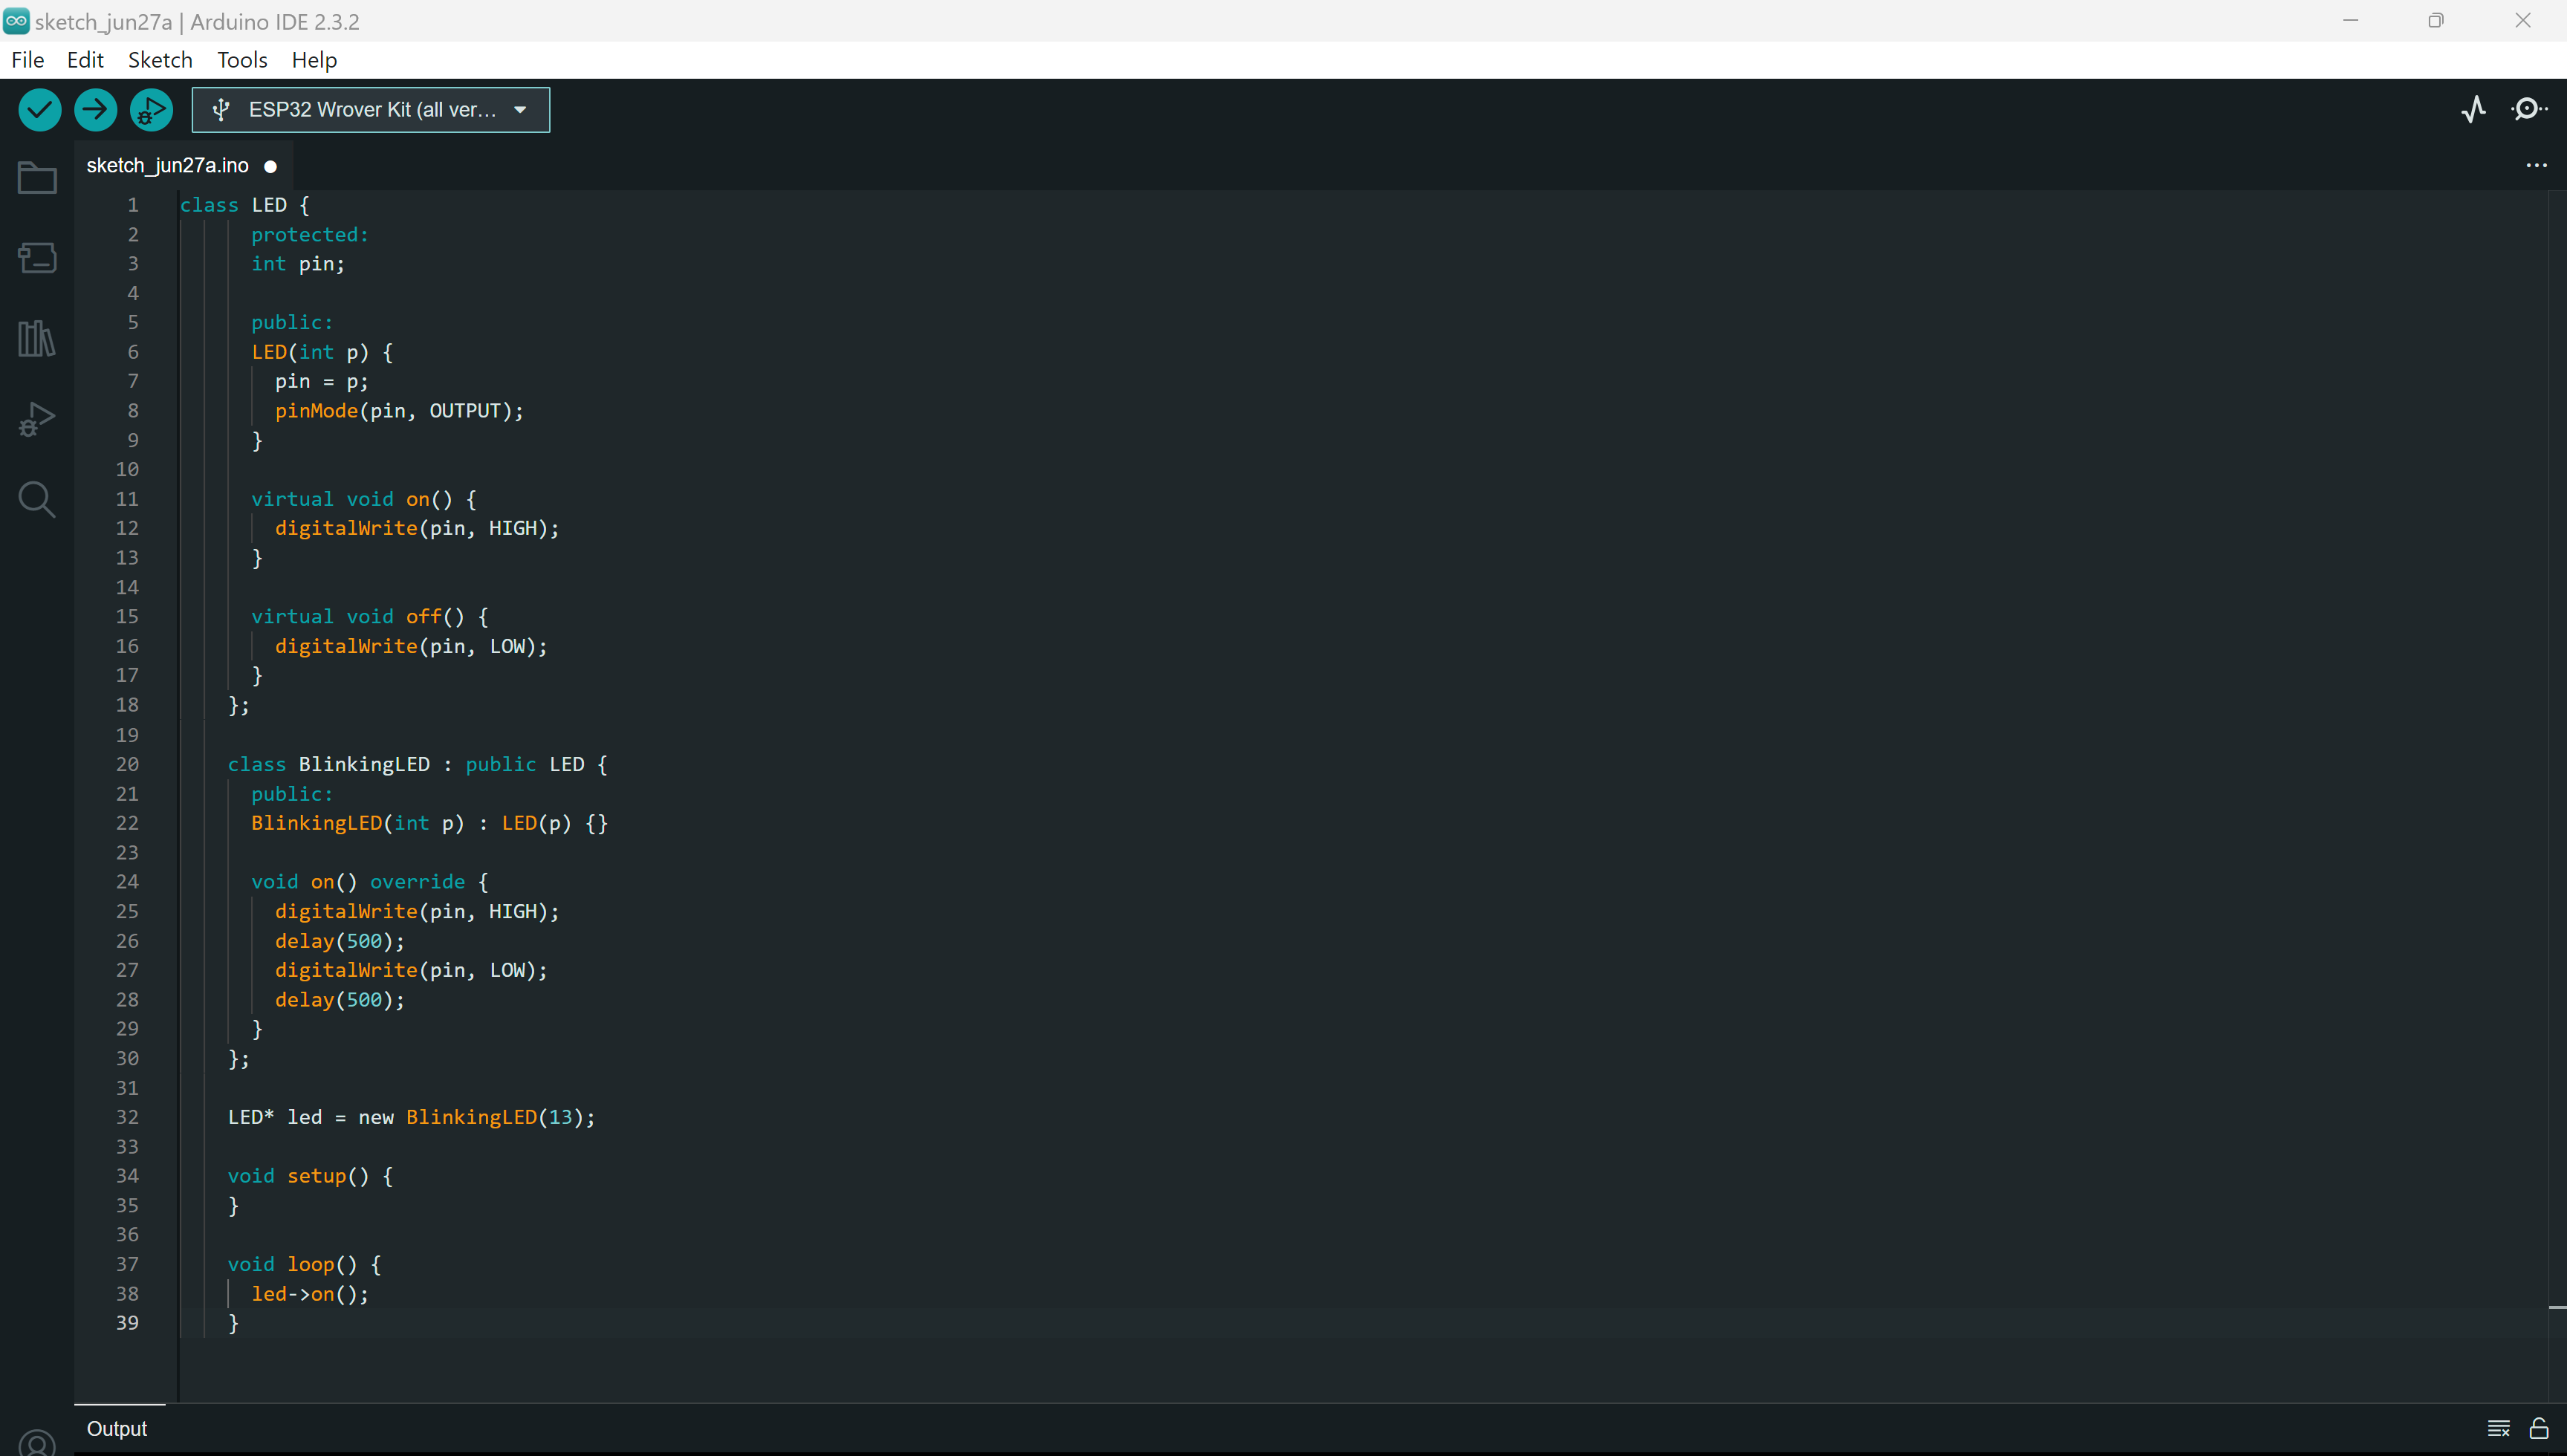
\includegraphics[width=\textwidth]{fig/fig20.png}
	\caption{text}
	\label{fig:20}
\end{figure}

\chapter{Opgave}
\textbf{Opgave:} Lav et Arduino-program, der bruger en klasse til at styre en LED. Klassen skal have metoder til at tænde, slukke og blinke LED'en. Brug en knap til at skifte mellem at tænde, slukke og blinke LED'en.
\begin{itemize}
	\item Opret en klasse \texttt{LED} med metoderne \texttt{on()}, \texttt{off()} og \texttt{blink()}.
	\item Brug en knap til at skifte mellem tilstande (tændt, slukket, blinkende).
	\item Brug \texttt{digitalRead()} til at læse knapstatus.
	\item Brug \texttt{digitalWrite()} til at styre LED'en.
\end{itemize}
\clearpage
\noindent\textbf{Løsningsforslag:}
\begin{lstlisting}[language=C++]
	class LED {
		int pin;
		
		public:
		// Constructor to initialize the LED pin
		LED(int p) {
			pin = p;
			pinMode(pin, OUTPUT);
		}
		
		// Turn the LED on
		void on() {
			digitalWrite(pin, HIGH);
		}
		
		// Turn the LED off
		void off() {
			digitalWrite(pin, LOW);
		}
		
		// Blink the LED with a 500ms delay (blocking function)
		void blink() {
			on();
			delay(500);
			off();
			delay(500);
		}
	};
	
	LED led(13);             // Create an LED object on pin 13
	int buttonPin = 2;       // Button input pin
	int buttonState = 0;     // Current state of the button
	int ledState = 0;        // 0: off, 1: on, 2: blink
	
	void setup() {
		pinMode(buttonPin, INPUT); // Initialize the button pin as input
	}
	
	void loop() {
		buttonState = digitalRead(buttonPin); // Read the button state
		
		// Check if the button is pressed
		if (buttonState == HIGH) {
			ledState = (ledState + 1) % 3; // Cycle through LED states
			delay(200); // Debounce delay (consider reducing to ~50-100ms)
		}
		
		// Handle the LED state
		switch (ledState) {
			case 0:
			led.off(); // Turn off the LED
			break;
			case 1:
			led.on();  // Turn on the LED
			break;
			case 2:
			led.blink(); // Blink the LED
			break;
		}
	}
\end{lstlisting}
